\documentclass[tikz,border=6pt]{standalone}
\usepackage{fontspec}
\setmainfont{Noto Sans}
\usepackage{amsmath,amssymb}
\usepackage{tikz}
\usetikzlibrary{arrows.meta,positioning}
\definecolor{cudaG}{RGB}{118,185,0}
\definecolor{gsBlue}{RGB}{40,110,190}
\definecolor{secG}{RGB}{85,85,85}

\begin{document}
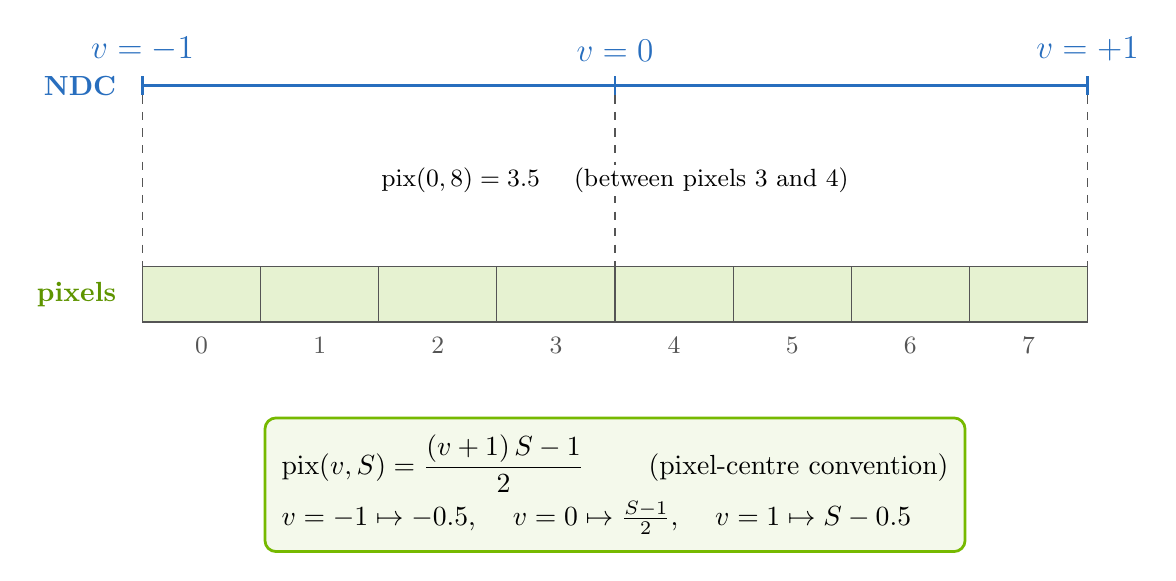
\begin{tikzpicture}[x=1.5cm,y=1cm, every node/.style={font=\large}]
  % S = 8 pixels (illustrative). Pixel centres at integer pixel coordinates 0..7.
  % Map: x = (v+1)*4 for NDC, x = pix + 0.5 for pixels (so pixel i spans [i,i+1]).

  % NDC axis
  \draw[very thick, gsBlue] (0,3) -- (8,3);
  \foreach \v/\lab in {-1/{-1},0/{0},1/{+1}} {
    \pgfmathsetmacro{\xx}{(\v+1)*4}
    \draw[thick, gsBlue] (\xx,3.12) -- (\xx,2.88);
    \node[above=2pt, gsBlue] at (\xx,3.12) {$v=\lab$};
  }
  \node[left=6pt, gsBlue, font=\bfseries] at (0,3) {NDC};

  % Pixel row
  \foreach \i in {0,...,7} {
    \fill[cudaG!18] (\i,0) rectangle (\i+1,0.7);
    \draw[secG] (\i,0) rectangle (\i+1,0.7);
    \node[below=2pt, font=\small, secG] at (\i+0.5,0) {$\i$};
  }
  \node[left=6pt, cudaG!80!black, font=\bfseries] at (0,0.35) {pixels};

  % Mapping lines from NDC to pixel edges (v=-1, 0, 1)
  \foreach \xx/\lab in {0/{$\text{pix}=-0.5$},4/{$\text{pix}=3.5$},8/{$\text{pix}=7.5$}} {
    \draw[dashed, secG] (\xx,2.88) -- (\xx,0.7);
  }
  \node[font=\small, fill=white, inner sep=1pt] at (4,1.8) {$\text{pix}(0,8)=3.5$ \quad (between pixels 3 and 4)};

  % Formula box
  \node[draw=cudaG, line width=1pt, rounded corners, fill=cudaG!8, inner sep=6pt,
        anchor=north, align=left, font=\normalsize] at (4,-1.2)
        {$\text{pix}(v,S)=\dfrac{(v+1)\,S-1}{2}$ \qquad (pixel-centre convention)\\[2pt]
         $v=-1\mapsto -0.5$, \quad $v=0\mapsto \tfrac{S-1}{2}$, \quad $v=1\mapsto S-0.5$};
\end{tikzpicture}
\end{document}
